\section{Frontend} \label{frontend}
Frontend slouží jako nástroj pro vizualizaci aplikace. Patří sem veškeré soubory pro vykreslování stránek, obrázky, mapa a grafy. Uživatel může jednoduše přepínat mezi stránky aplikace, kterými jsou: domovská stránka, mapa a údaje o vývojářích.

Frontend aplikace obsahuje soubory vue.js, což je javascriptový framework, který se stará o dynamické a reaktivní zobrazení uživatelského rozhraní. Vue.js je velmi populární a používaná technologie i velkými firmami, která funguje na bázi jednoduchých šablon a komponent.
Vue.js je nováčkem na trhu, ale disponuje rychlostí a velkými možnostmi oproti ostatním frameworkům.
Tato technologie usnadňuje uživatelům jednoduché použití a přehlednou dokumentací. Kvůli rozsáhlému používání jsme usoudili, že vue.js je správná volba. 

Pro odbavování HTTP požadavků jsme použili knihovnu axios, která propojuje backend s frontendem na základě jejich požadavkům. Disponuje rychlostí, jednoduchým odbavováním a odesíláním požadavků a propracovanou dokumentací, která je základem pro správné použití.
Jde o technologii používanou všemi úrovni vývojářů. Aplikace umožňuje odesílání asynchroních požadavků, transformací dat a správou případných chyb.
Za pomocí čtení url stránky posílá axios odpověď. Tímto způsobem se dostanou data z databáze až do grafů na frontendu. 
Pro vykreslení mapy s body jsme zvolili knihovnu leaflet, která je podrobně popsána v kapitole mapa stanic. Pro zpracování grafů jsme zvolili knihovnu chart.js, která je popsána v kapitole grafy.

\subsection{Grafy}
%\cite{grafy_chartsjs}
Pro přehledné vykreslení dat jsme zvolili grafy. Na stránce je vykresleno pět grafů podle jejich typu(teplota, déšť, rychlost větru, směr větru, tlak). %\ref ukazka_grafu

Na ose x jsou zobrazeny časové údaje a ose y hodnoty pro daný čas. Použité grafy jsou z opensource knihovny charts.js, která umožňuje přehledně a jednoduše grafy nastylizovat a upravovat dle potřeb.

Uživatel má možnost měnit časový úsek vykreslení dat pomocí tlačítka pod souřadnicemi stanice. Na výběr má z předdefinovaných hodnot (např. den, týden, rok), ale pomocí výběru "vlastní" si může nastavit své vlastní časové rozmezí.
Pro rozpoznání grafů je nad každým grafem jméno, které určuje, co je v daném grafu ukázáno. Grafem je křivka, která plynule propojuje dva sousední body.  

Knihovna chart.js nebyla naší první volbou, jelikož jsme v předchozích verzích používali ApexCharts.js, ale knihovna nám nevyhovovala v možnostech vykreslení grafů, nekompletní dokumentací a její intuitivností ve smyslu implementování.
Z těchto důvodů jsme knihovnu nahradili charts.js, která má o poznání přehlednější dokumentaci a obsahuje více potřebných funkcí.

\begin{figure}[h] %screenshot grafu 
    \centering
    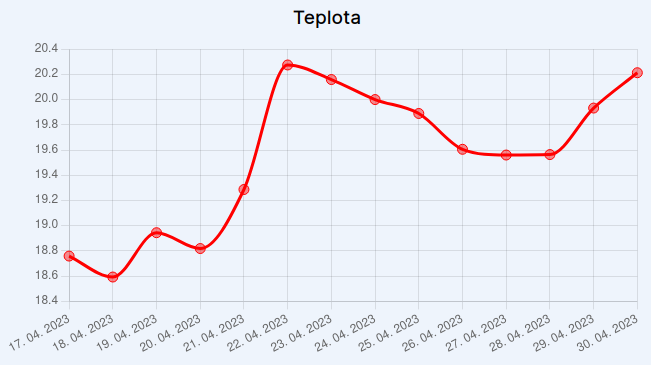
\includegraphics[width=0.25\textwidth]{images/graf.png}
    \caption{Graf s teplotami}
    \label{ukazka_grafu}
\end{figure}

\subsection{Mapa stanic}
Aby si mohl uživatel zobrazit data, musí se dostat na stránku s mapou, ve které je vidět bod. Po kliknutí na bod se dozví poslední naměřené údaje a může se prokliknout pomocí odkazu na podrobnější údaje v podobě grafů.

Pro vykreslení bodů do mapy jsme použili opensource knihovnu leaflet.js, která disponuje velkou škálou možností pro vykreslení bodů, množin a tvarů.
Avšak vybrání této knihovny také nebylo jednoduché. Prvoplánově jsme zamýšleli použít známé mapy jako jsou google maps nebo apple maps, ale implementace těchto knihoven byla pro naše účely zbytečně složitá. Dále tyto knihovny obsahují zdlouhavě a neintuitivní dokumentace, což je při práci s nimi nepříjemné.
Knihovna leaflet je populární a rozsáhle používána pro mobilní aplikace. Použití této mapy lze pozorovat například u dopravce české dráhy, sociální sítě Facebook a flickr.

\begin{figure}[h] %screenshot grafu 
    \centering
    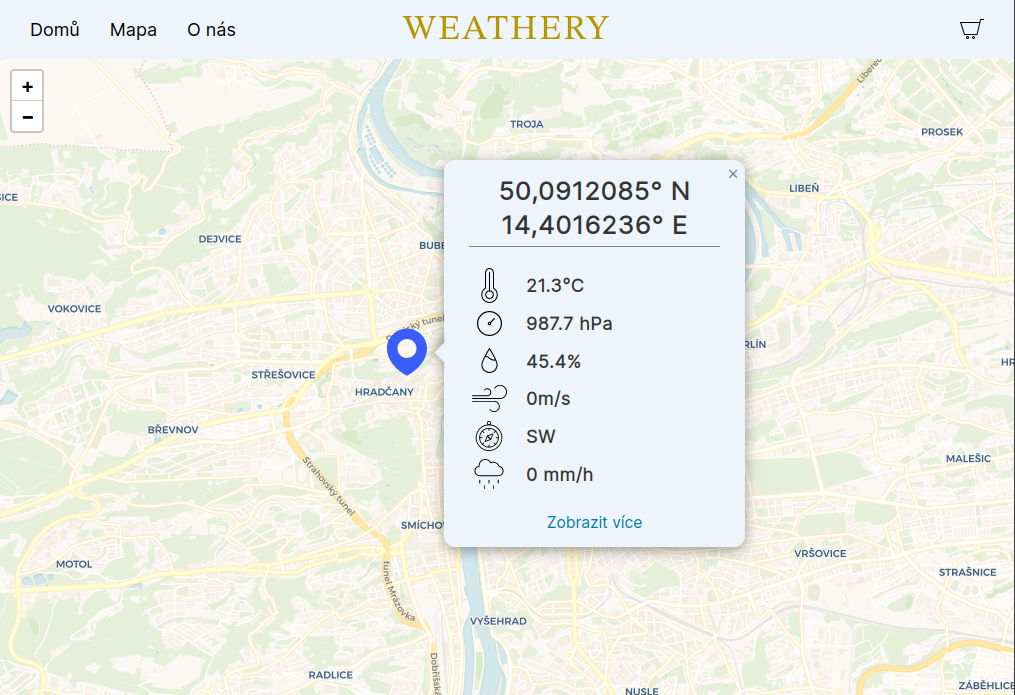
\includegraphics[width=0.25\textwidth]{images/mapa.png}
    \caption{Mapa stanic}
    \label{mapa}
\end{figure}


Pro nastavení mapy jsme zvolili světlé pozadí s málo kontrastním vykreslením vodních ploch, obytných oblastí, silnic, přírodních míst a hranic států. Uživatel má možnost libovolně mapu oddalovat a přibližovat, přičemž výchozím bodem mapy je Praha, na kterou je mapa po spuštění zaměřená.

\subsection{Design}
Design znamená vizuální podoba stránky.
Naším cílem bylo vytvořit intuitivní prostředí pro uživatele, ve kterém se dokáže rychle a jednoduše pohybovat.

Prvním setkáním s designem webu je domovská stránka, která obsahuje funkci detekující kolečko myši.
Právě tímto pohybem se stránka odhaluje a postupně mění. V průběhu animace se uživatel dozví informace o dlouhodobějších změnách počasí a srovnání počasí napříč roky.

%About us 
Na stránce nákup se uživatel dozví podobu stanice a je obeznámen s registrací a podrobnostmi.

\begin{figure}[h] %screenshot grafu 
    \centering
    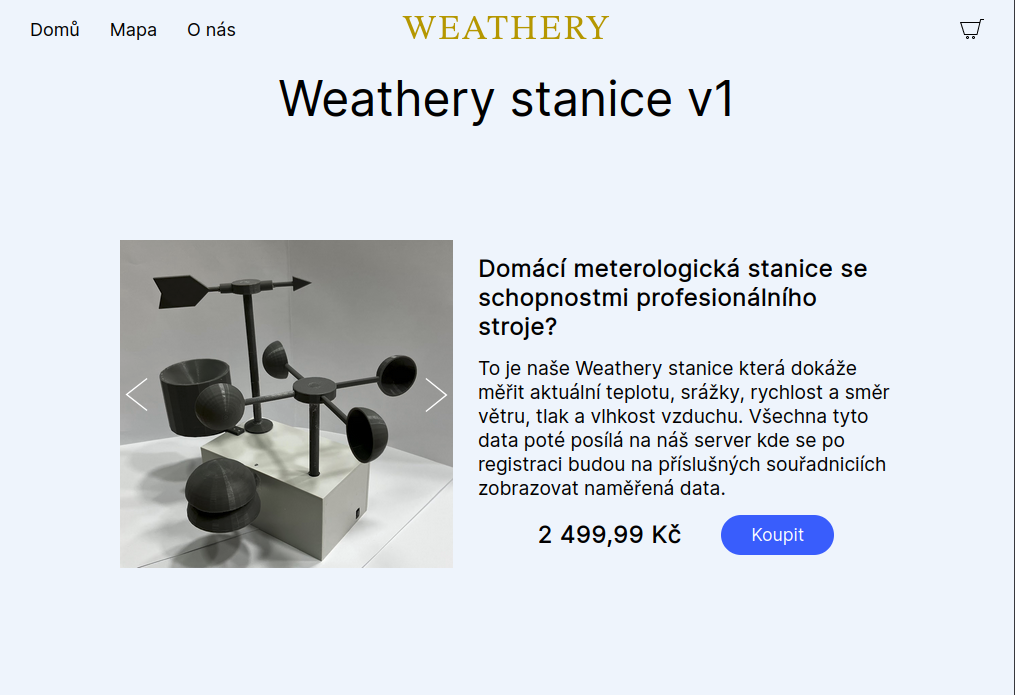
\includegraphics[width=0.25\textwidth]{images/nakup.png}
    \caption{Nákup stanice}
    \label{nakup}
\end{figure}
